% !TeX spellcheck = en_GB

\section{Ensemble spread}%\hfill} 
\label{app:ens_spread}

%%% image ensemble spread %%%%%%%%%%%%%%%%%%%%%%%%%%%%%%%%%%%%%
\begin{figure}[h!]
	\centering
	% 20/12
	\begin{subfigure}[t]{\textwidth}		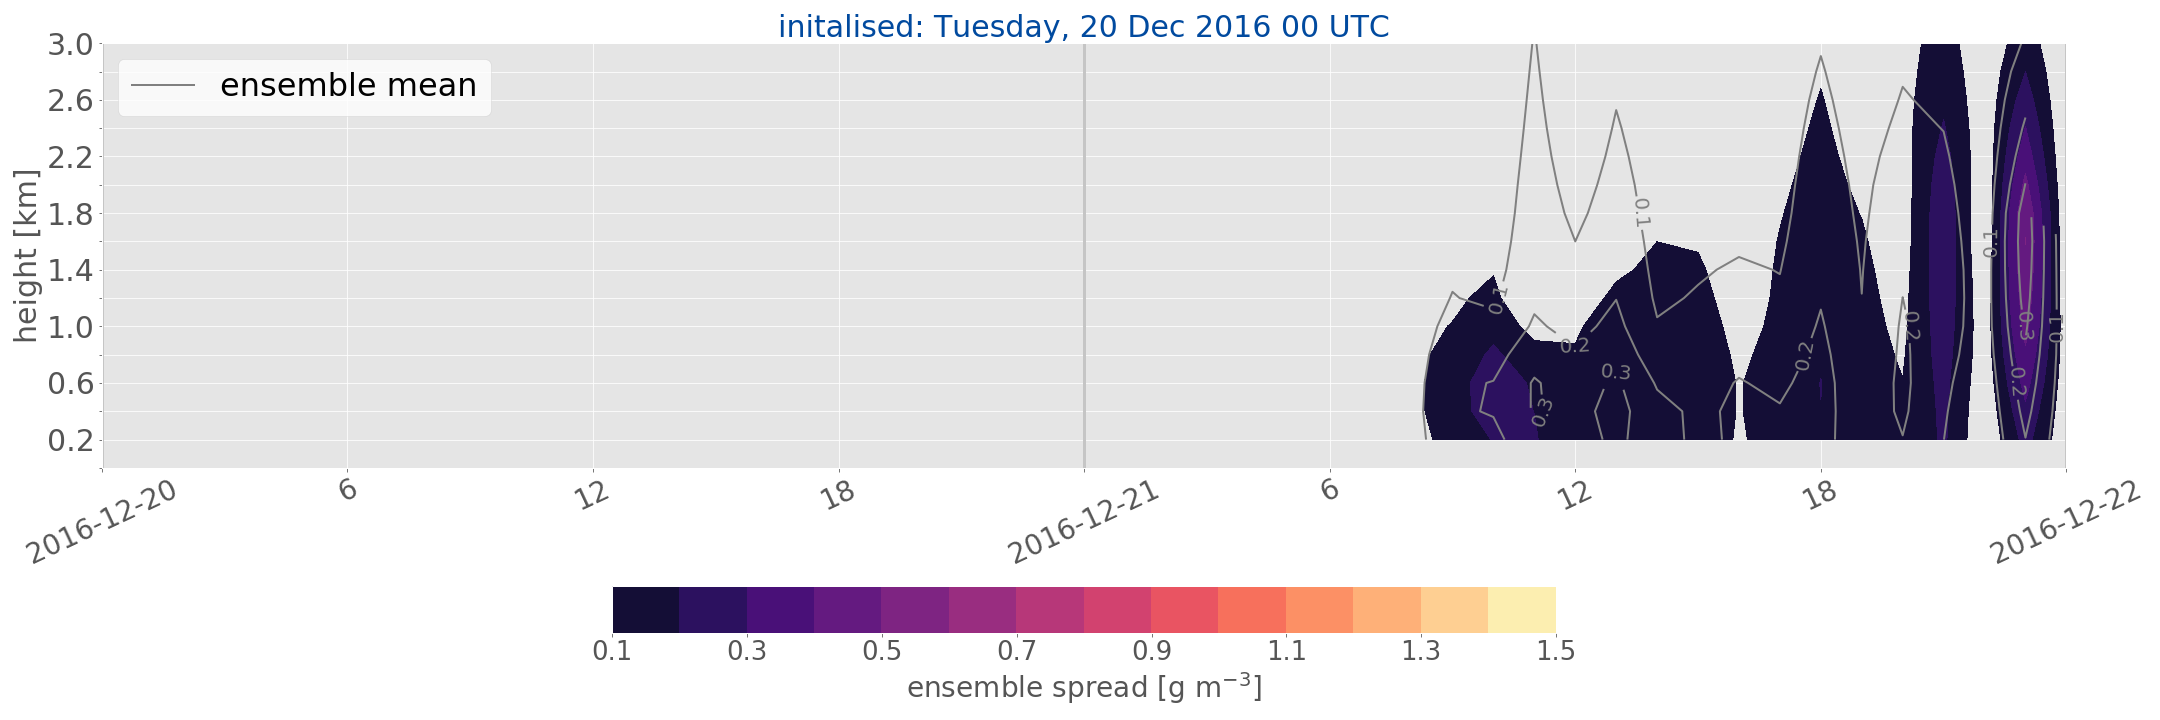
\includegraphics[trim={0.cm 5.3cm 0cm 0cm},clip,width=\textwidth]{./fig_ensemble_spread/20161220}
		\caption{}\label{fig:ens_spread20}
	\end{subfigure}
	% 21/12
	\begin{subfigure}[t]{\textwidth}		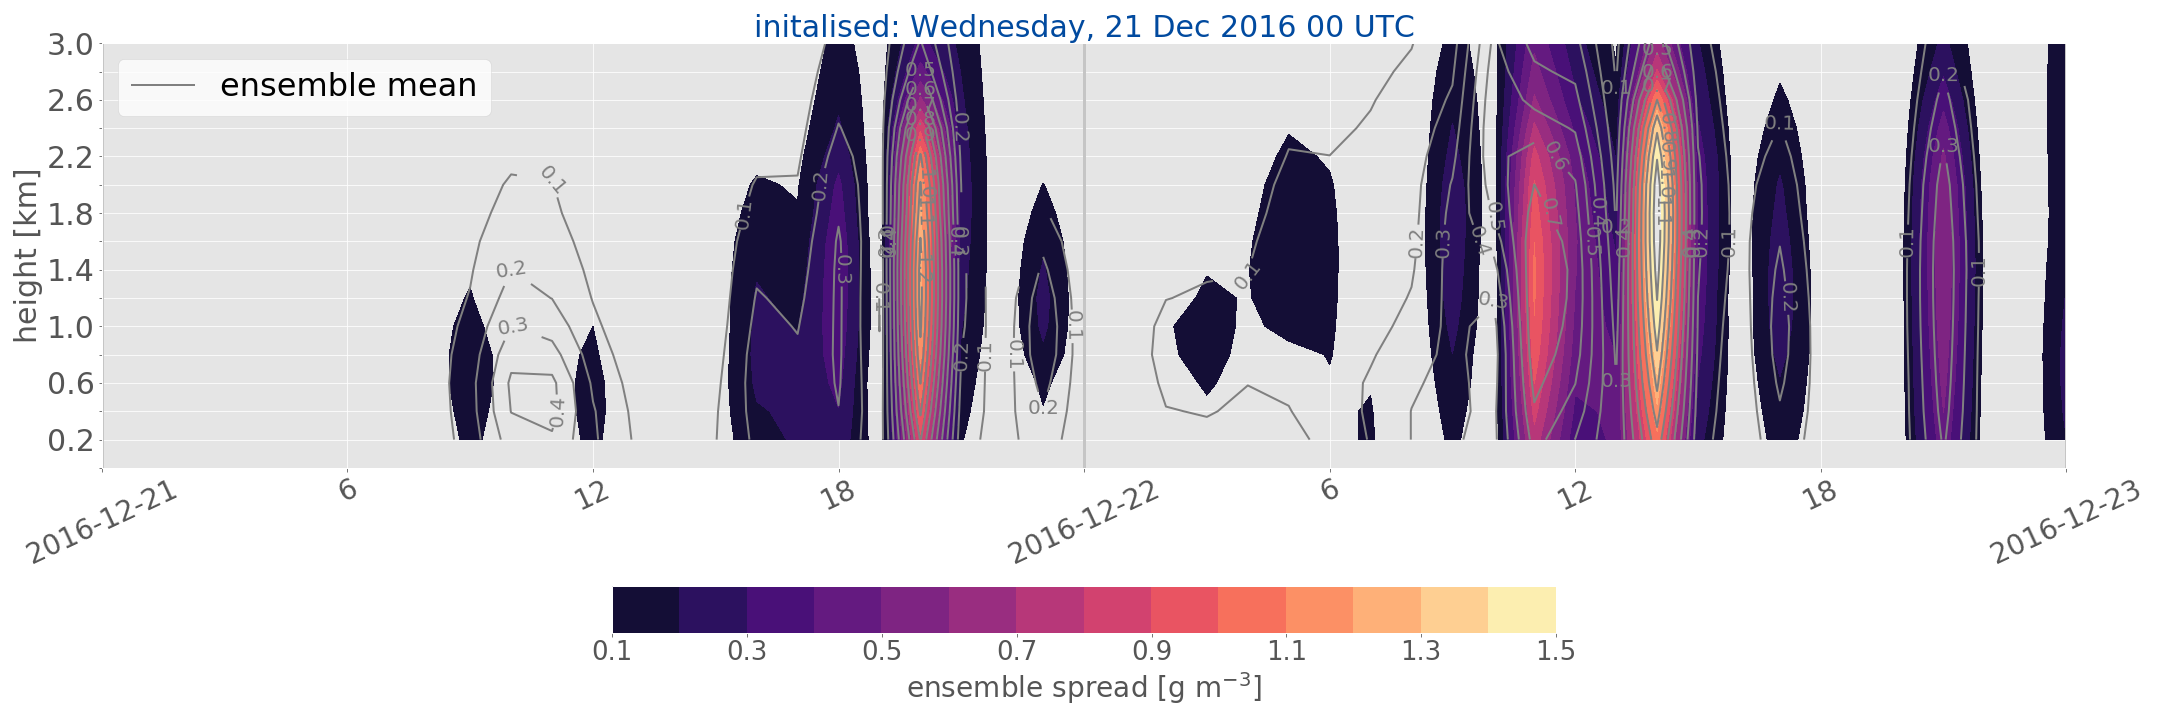
\includegraphics[trim={0.cm 5.3cm 0cm 0cm},clip,width=\textwidth]{./fig_ensemble_spread/20161221}
		\caption{}\label{fig:ens_spread21}
	\end{subfigure}
	% colourbar
	\begin{subfigure}[t]{\textwidth}		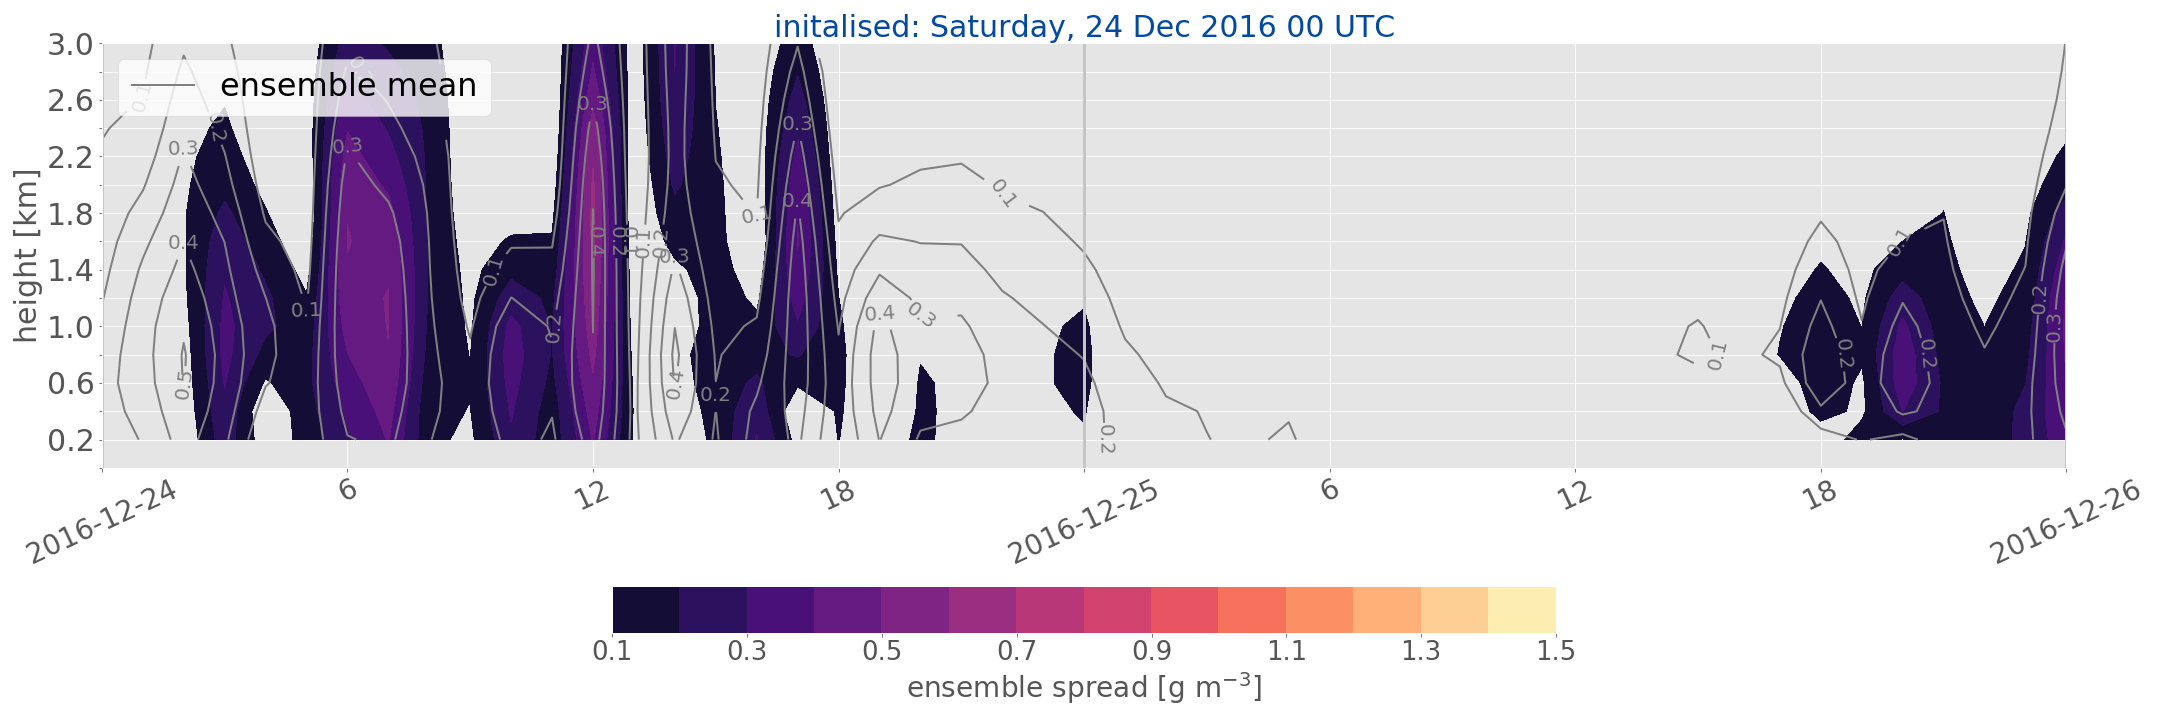
\includegraphics[trim={15.cm 0cm 15cm 21cm},clip,width=\textwidth]{./fig_ensemble_spread/20161224}
	\end{subfigure}
\end{figure}
\begin{figure}[t]\ContinuedFloat        
	% 22/12
	\begin{subfigure}[t]{\textwidth}		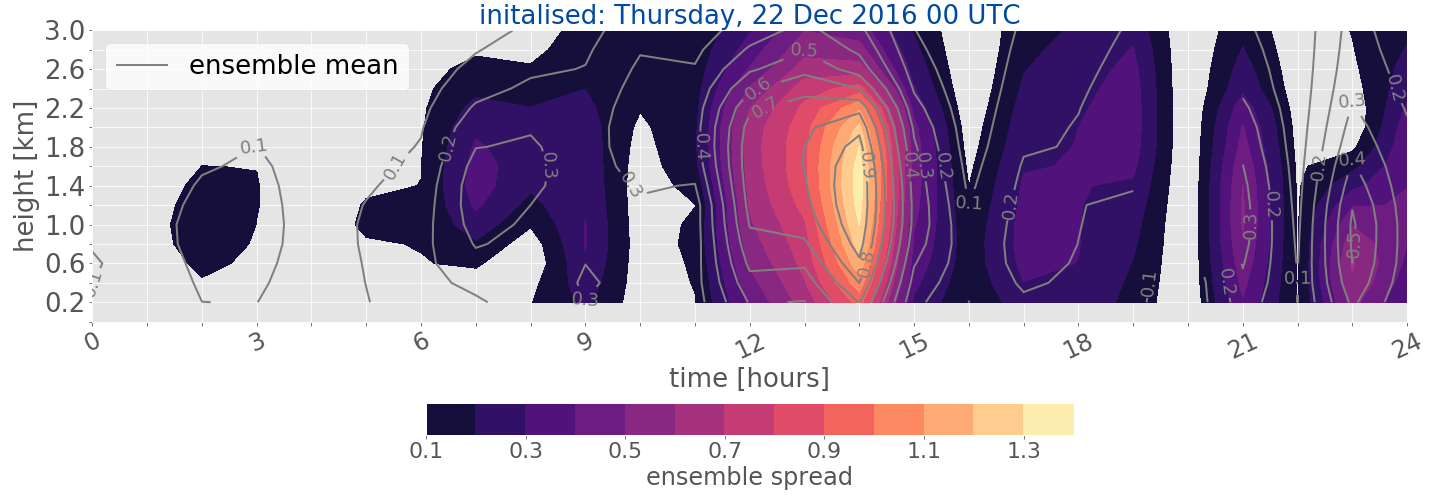
\includegraphics[trim={0.cm 5.3cm 0cm 0cm},clip,width=\textwidth]{./fig_ensemble_spread/20161222}
		\caption{}\label{fig:ens_spread22}
	\end{subfigure}
	% 23/12
	\begin{subfigure}[t]{\textwidth}		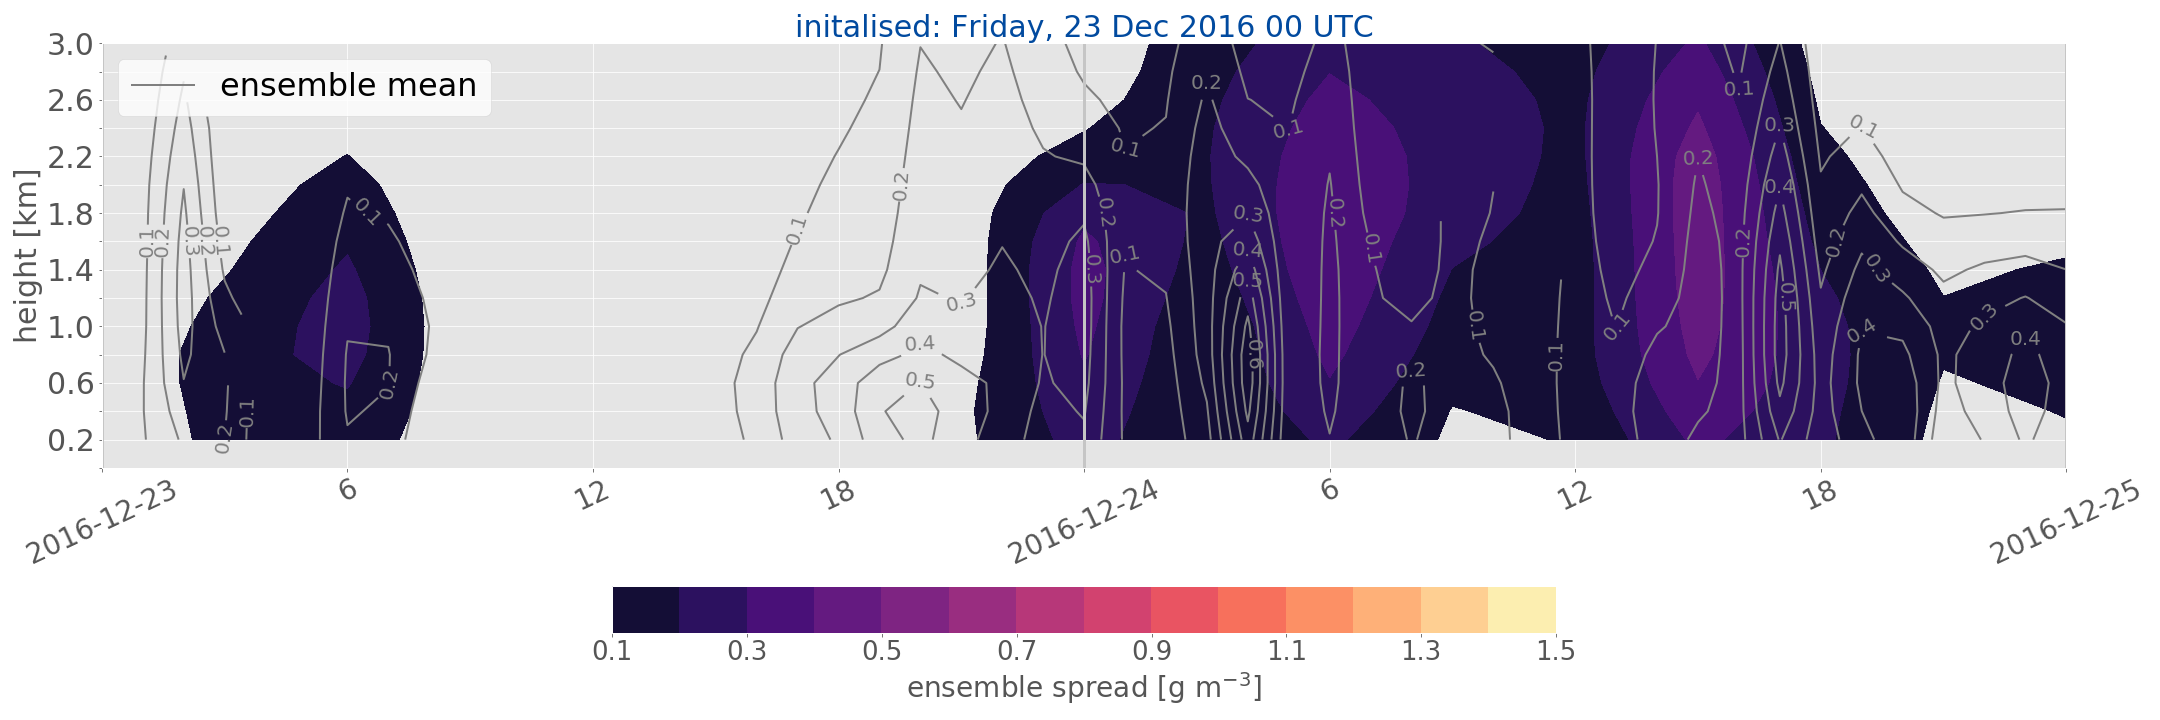
\includegraphics[trim={0.cm 5.3cm 0cm 0cm},clip,width=\textwidth]{./fig_ensemble_spread/20161223}
		\caption{}\label{fig:ens_spread23}
	\end{subfigure}   
	% 24/12
	\begin{subfigure}[t]{\textwidth}		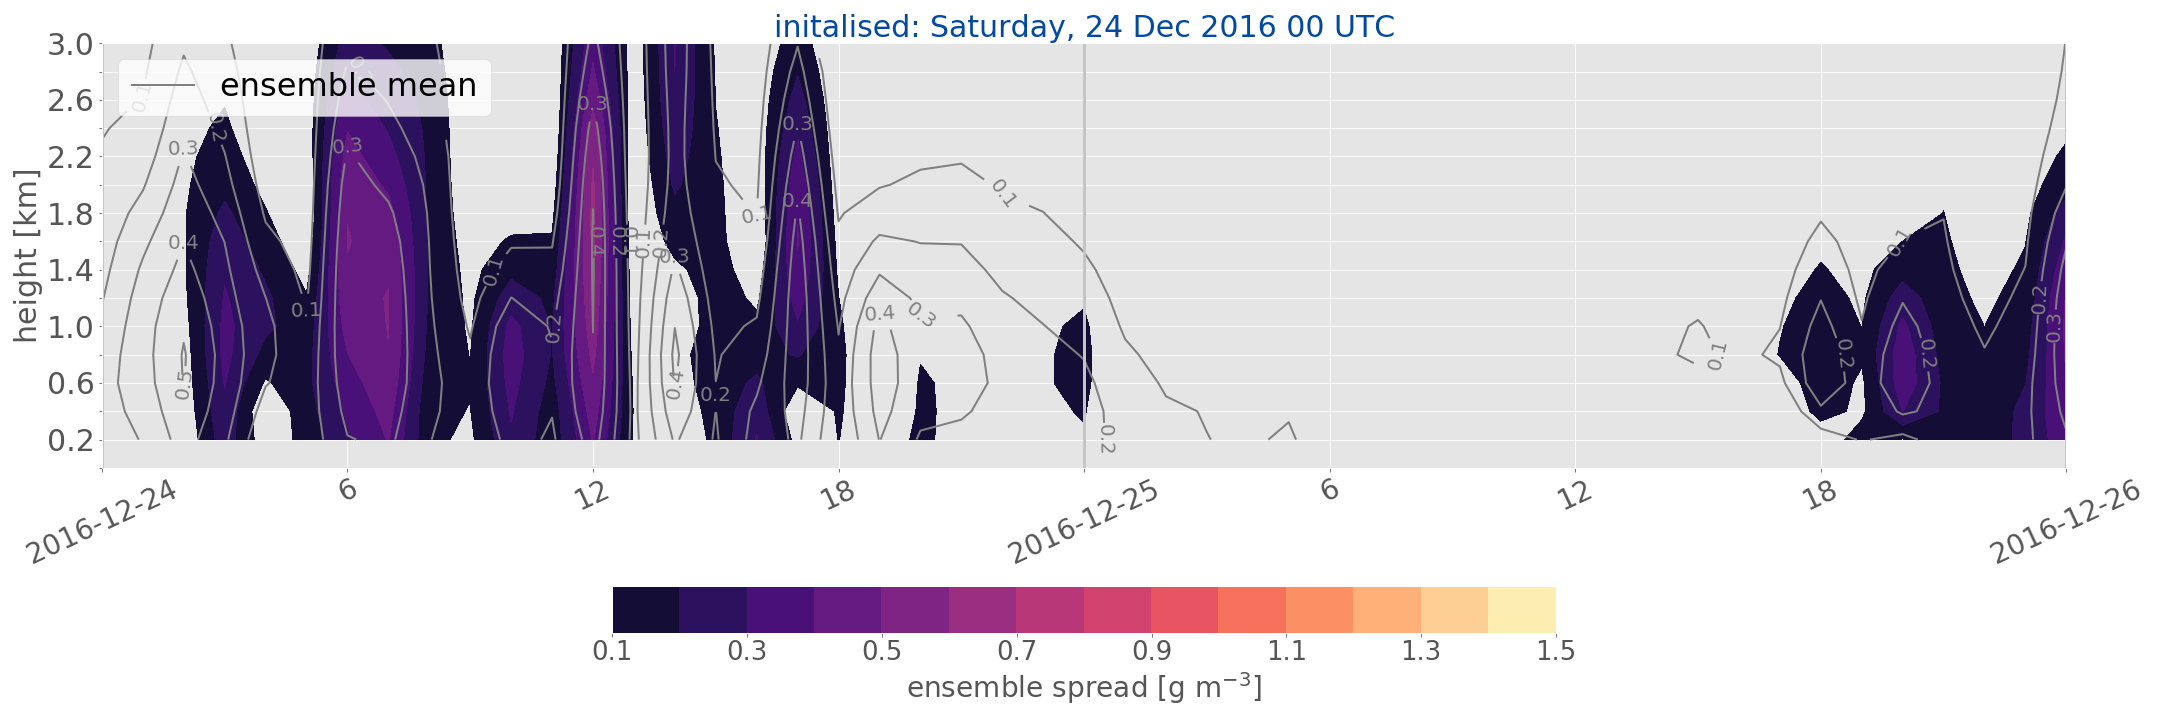
\includegraphics[trim={0.cm 5.3cm 0cm 0cm},clip,width=\textwidth]{./fig_ensemble_spread/20161224}
		\caption{}\label{fig:ens_spread24}
	\end{subfigure}        
	% colourbar
	\begin{subfigure}[t]{\textwidth}		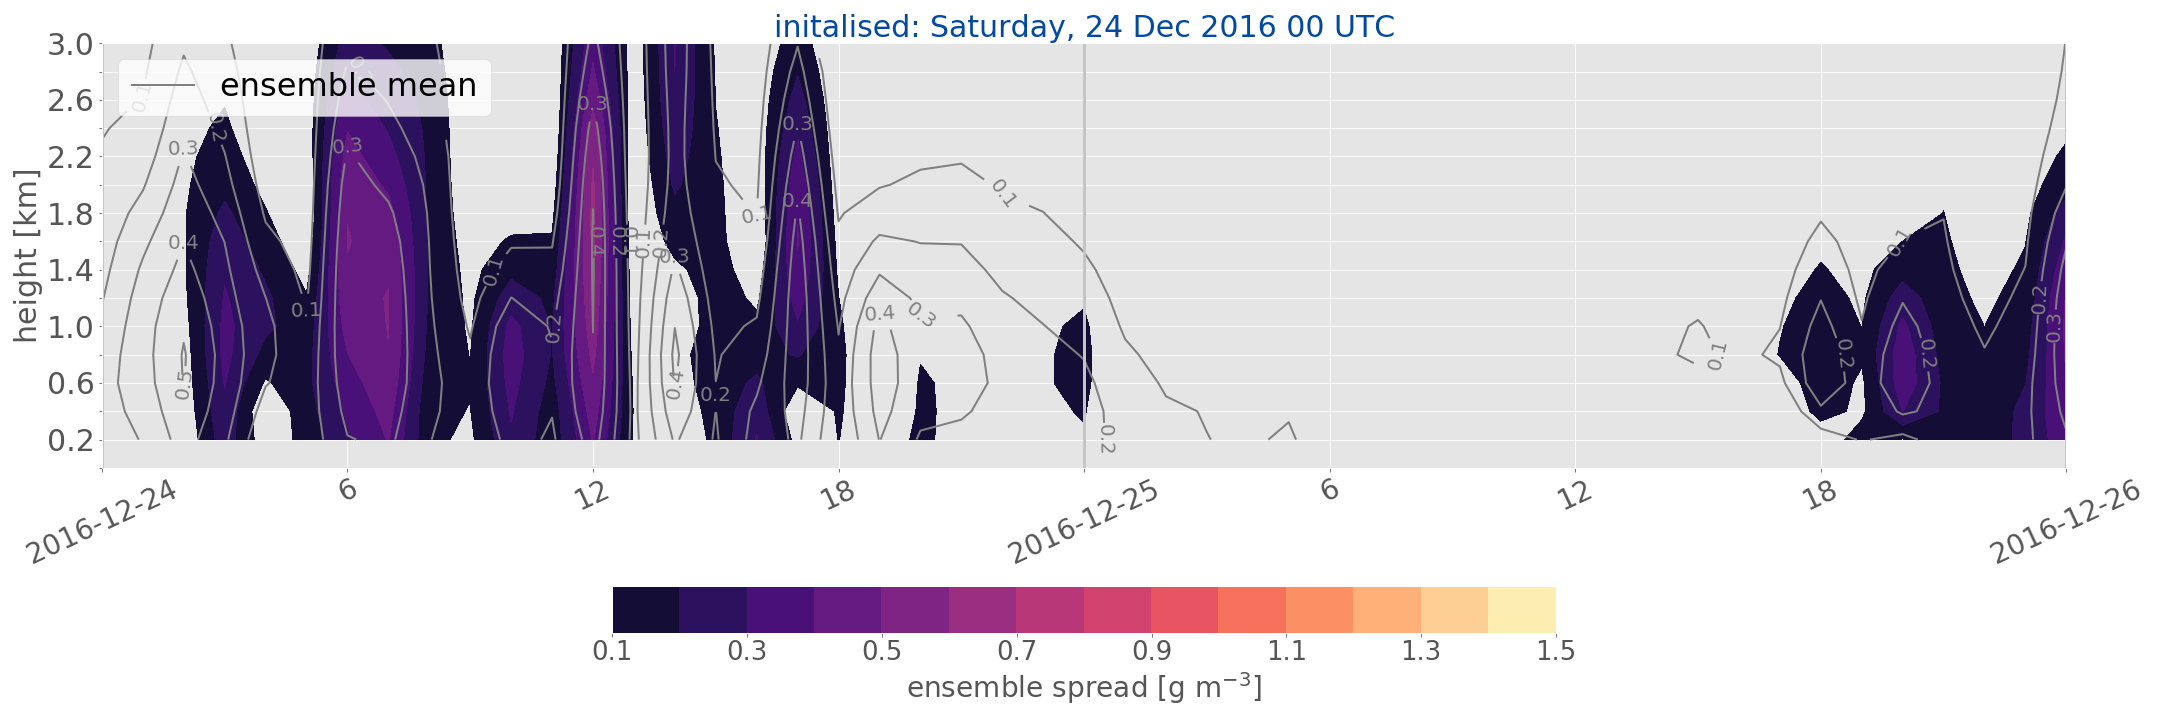
\includegraphics[trim={15.cm 0cm 15cm 21cm},clip,width=\textwidth]{./fig_ensemble_spread/20161224}
	\end{subfigure}
\end{figure}
\begin{figure}[t]\ContinuedFloat
	\centering
	% 25/12
	\begin{subfigure}[t]{\textwidth}		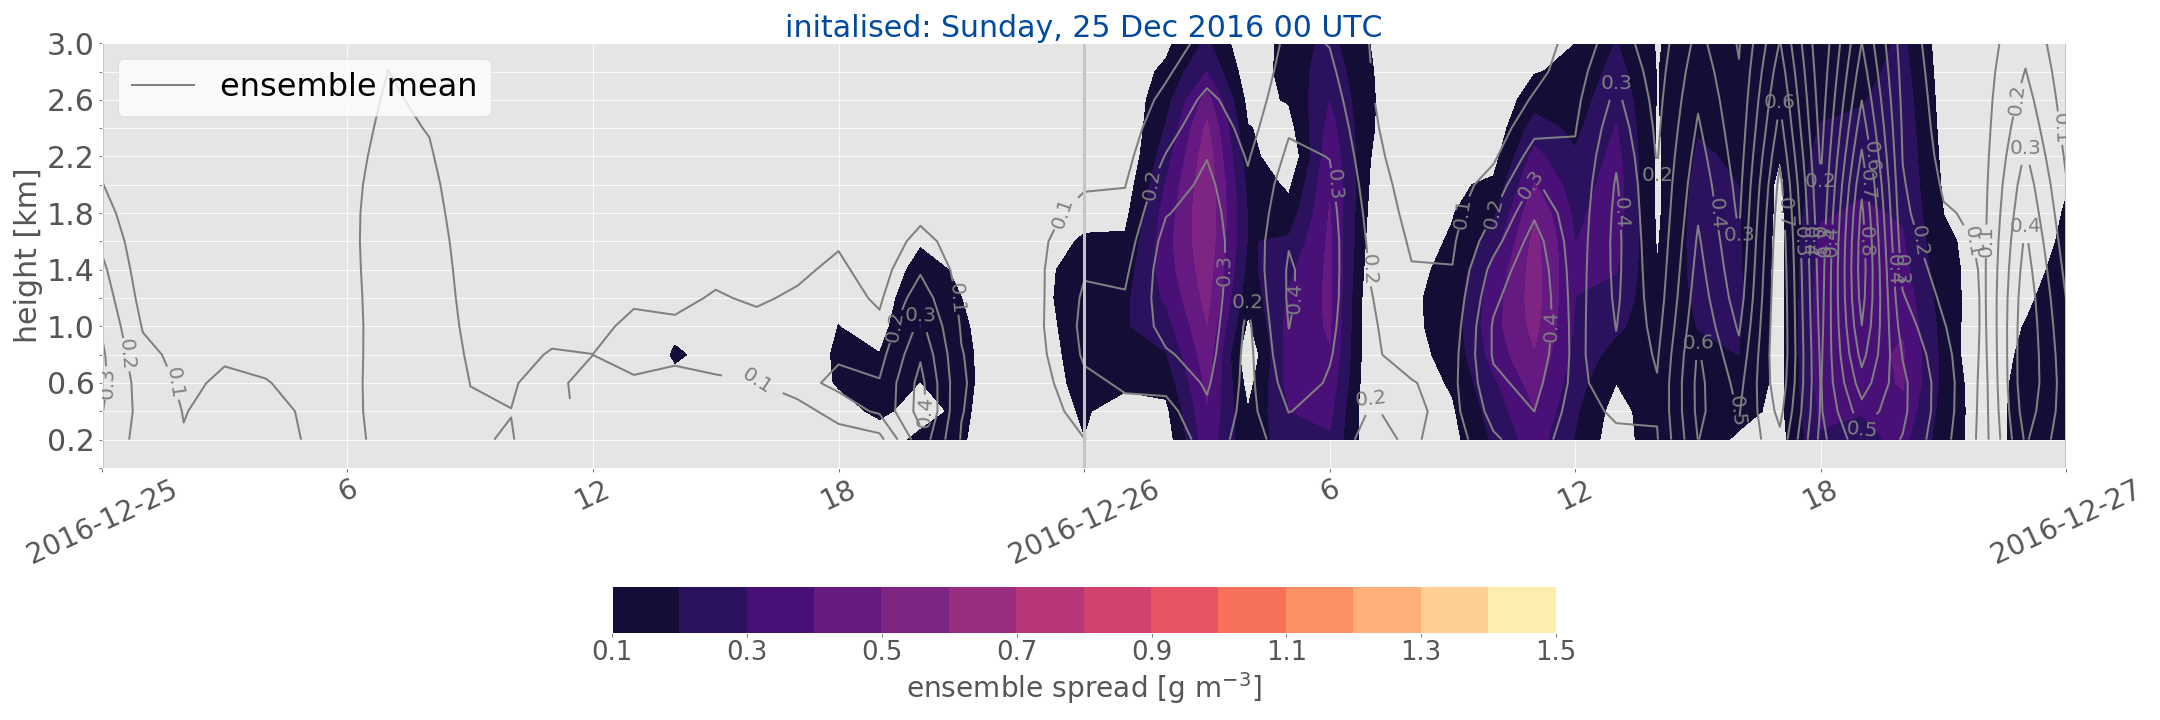
\includegraphics[trim={0.cm 5.3cm 0cm 0cm},clip,width=\textwidth]{./fig_ensemble_spread/20161225}
		\caption{}\label{fig:ens_spread25}
	\end{subfigure}
	% 26/12
	\begin{subfigure}[t]{\textwidth}		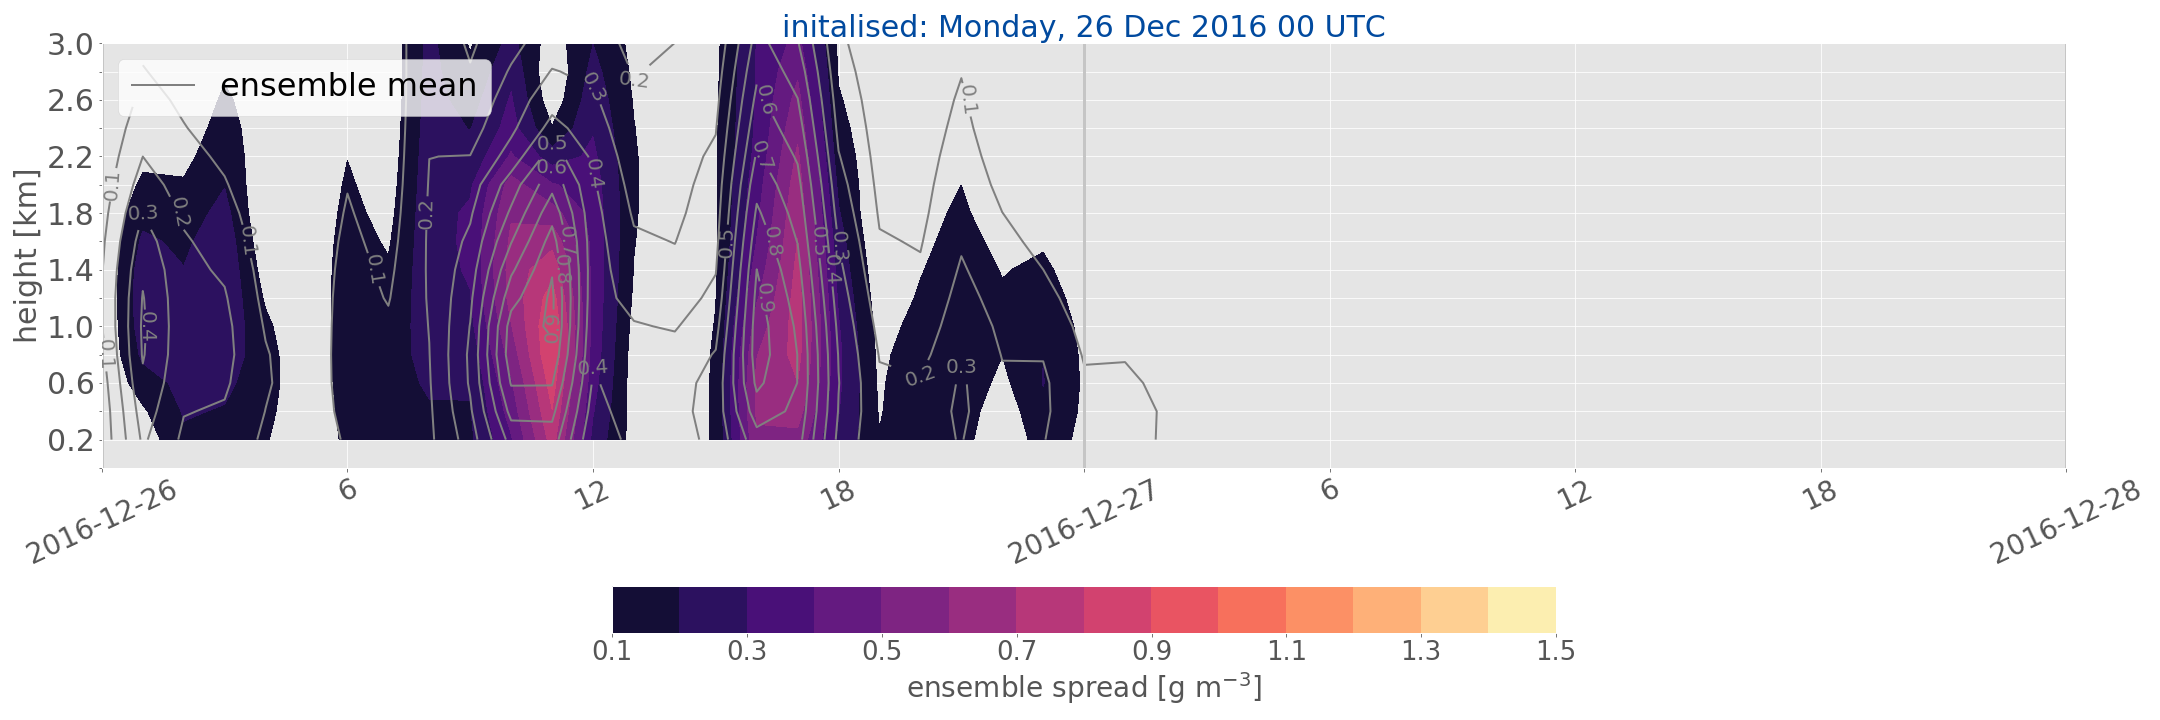
\includegraphics[trim={0.cm 5.3cm 0cm 0cm},clip,width=\textwidth]{./fig_ensemble_spread/20161226}
		\caption{}\label{fig:ens_spread26}
	\end{subfigure}
	% colourbar
	\begin{subfigure}[t]{\textwidth}		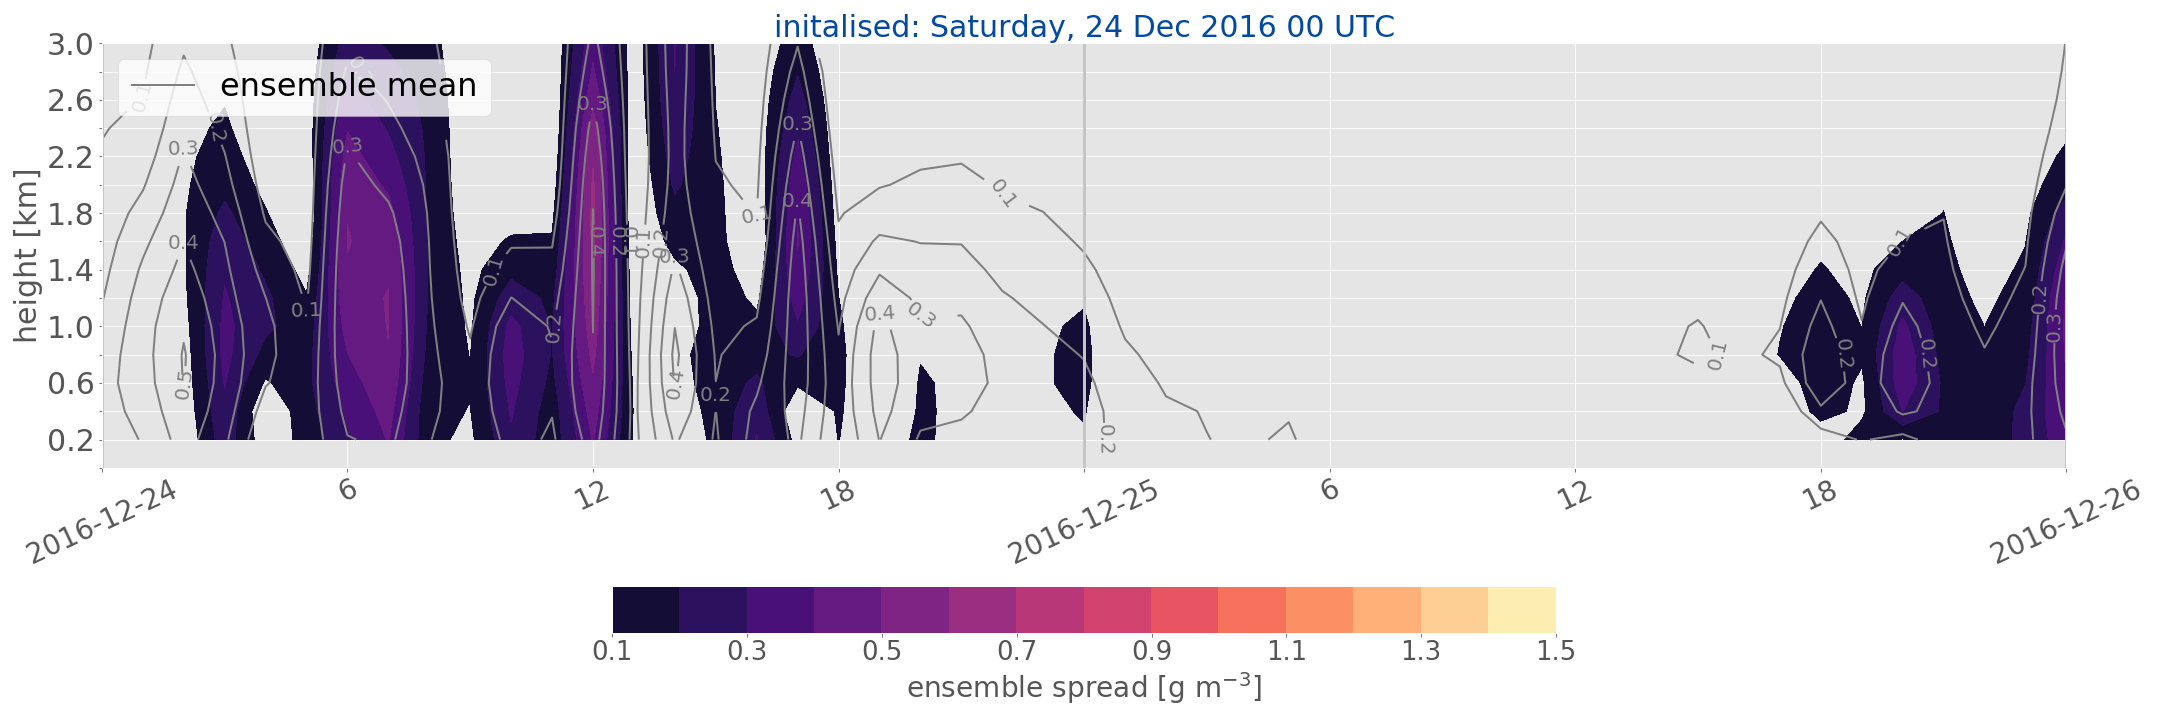
\includegraphics[trim={15.cm 0cm 15cm 21cm},clip,width=\textwidth]{./fig_ensemble_spread/20161224}
	\end{subfigure}
	\caption{Ensemble spread of the SWC of the ten ensemble members of MEPS. The lighter the colour according to the colour bar the higher the standard deviation between the perturbed ensemble members. In grey the ensemble mean of all ten members.}\label{fig:ens_spread}
\end{figure}

%%%%%%%%%%%%%%%%%%%%%%%%%%%%%%%%%%%%%%%%%%%%%%%%%%%%%%%%%%%%%%%%%%%%%%%%%%
